% David
%=============================================
% Puntos 12-17: Trayectoria del mínimo, interpretación geométrica,
% relación visualización-optimización, región mínima,
% relación con fuente real y conclusión visual.
%=============================================

\begin{frame}{Interpretación Geométrica y Conclusión Visual}

    \begin{columns}[T]

        %===========================================
        % COLUMNA IZQUIERDA: Trayectoria del mínimo
        %===========================================
        \column{0.52\textwidth}

        \begin{block}{Trayectoria del mínimo en el plano $(x,y)$}
            \centering
            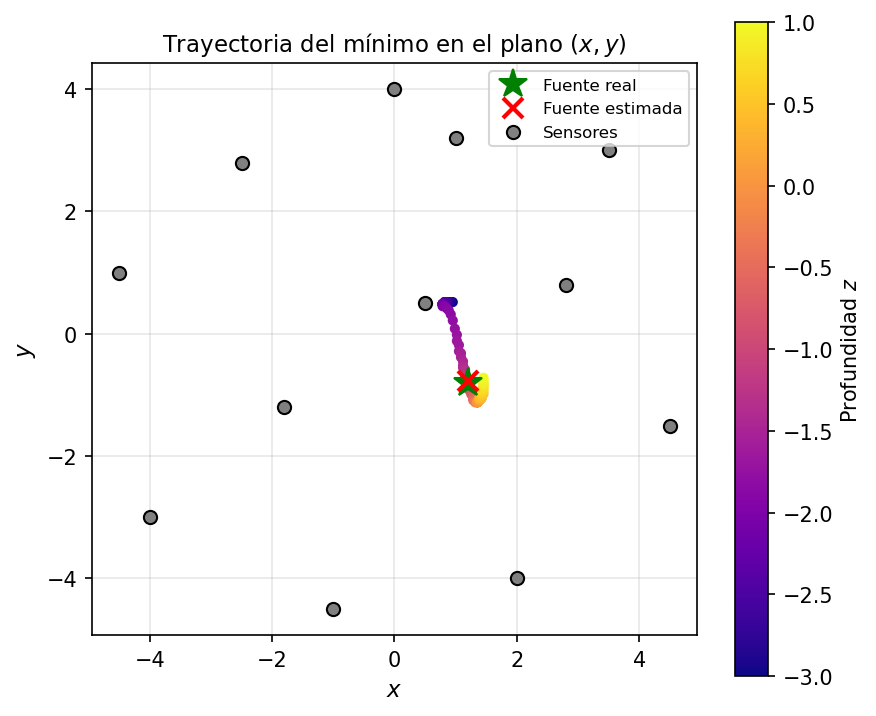
\includegraphics[width=0.92\textwidth]{Imagenes/trayectoria_minimo.png}
        \end{block}

        \vspace{0.1cm}
        \begin{center}
            \tiny \textcolor{gray}{Evolución de la posición del mínimo al variar la profundidad $z$.}
        \end{center}

        %===========================================
        % COLUMNA DERECHA: Interpretación y conclusión
        %===========================================
        \column{0.44\textwidth}

        \begin{block}{Interpretación Geométrica}
            \scriptsize
            \begin{itemize}
                \item La trayectoria muestra \textbf{cómo se desplaza} la ubicación estimada de la fuente al modificar $z$.
                \vspace{0.1cm}
                \item Las visualizaciones revelan la \textbf{forma de la superficie de error} y cómo el algoritmo converge hacia el mínimo.
                \vspace{0.1cm}
                \item La región mínima es la zona donde $A_{pred,i} \approx A_{obs,i}$ de manera más consistente.
            \end{itemize}
        \end{block}

        \vspace{0.2cm}

        \begin{exampleblock}{Relación con la Fuente Real}
            \scriptsize
            \begin{itemize}
                \item Las regiones de \textbf{menor error coinciden} con la ubicación real de la fuente simulada.
                \vspace{0.1cm}
                \item La visualización \textbf{confirma gráficamente} lo encontrado por el optimizador numérico.
            \end{itemize}
        \end{exampleblock}

    \end{columns}

    \vspace{0.15cm}
    \begin{center}
        \footnotesize
        \textbf{La visualización permite comprender intuitivamente cómo la optimización localiza la fuente sísmica.}
    \end{center}

\end{frame}